\documentclass[convert={density=300,outext=.png}]{standalone}
\usepackage{tikz}

\begin{document}
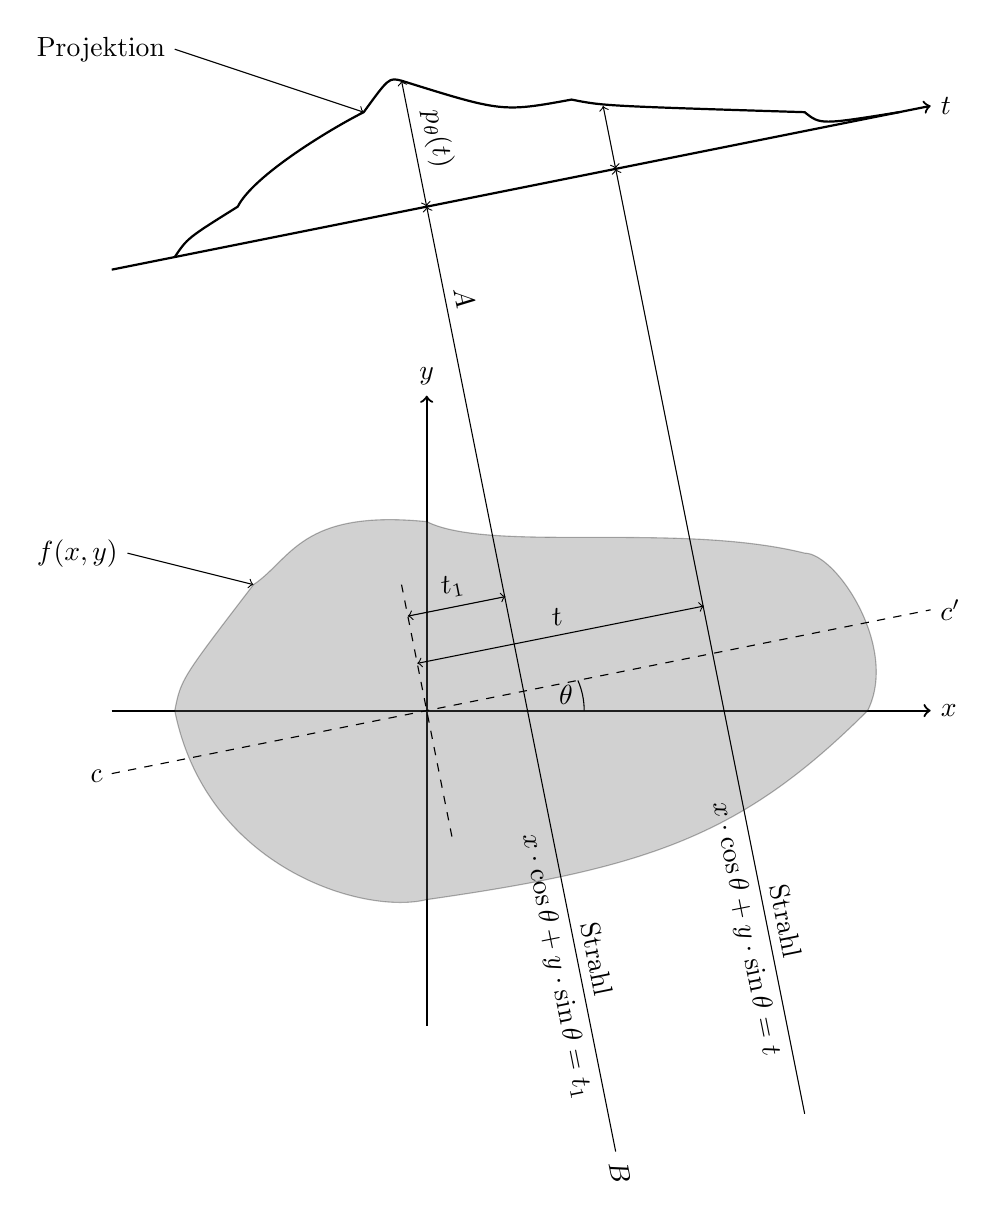
\begin{tikzpicture}[
    scale=0.8,
    axis/.style={thick,->}]
    % Achsen
    \draw[axis] (-5, 0) -- (8, 0) node[right] {$x$};
    \draw[axis] (0, -5) -- (0, 5) node[above] {$y$};
    \draw[axis] (-5, 7) -- (8, 9.6) node[right,sloped] {$t$};

    % Objekt
    \draw[fill=black!60!white,opacity=0.3] (0, -3) .. controls (3.5, -2.5) and (5, -2) .. (7, 0)
                                            .. controls (7.5, 1) and (6.5, 2.5) .. (6, 2.5)
                                            .. controls (4, 3) and (1, 2.5) .. (0,3)
                                            .. controls (-2, 3.2) and (-2.15, 2.4) .. (-2.75, 2)
                                            .. controls (-3.9, 0.5) .. (-4, 0)
                                            .. controls (-3.5, -2.5)  and (-1, -3.25) .. (0, -3);

    % Strahlen
    \draw[->] (3, -7) -- (0, 8) node[pos=0.9,above,sloped] {$A$} node[pos=0.2,above,sloped] {Strahl}
              node[pos=0.2,below,sloped] {$x \cdot \cos \theta + y \cdot \sin \theta = t_1$}
              node[pos=0,right,sloped] {$B$};

    \draw[->] (6, -6.4) -- (3, 8.6) node[pos=0.2,above,sloped] {Strahl}
              node[pos=0.2,below,sloped] {$x \cdot \cos \theta + y \cdot \sin \theta = t$};

    % t
    \draw[<->] (-0.3, 1.5) -- (1.25, 1.81) node[pos=0.5,above,sloped] {$t_1$};
    \draw[<->] (-0.15, 0.75) -- (4.4, 1.66) node[pos=0.5,above,sloped] {$t$};

    % sonstiges
    \draw[dashed] (-5, -1) -- (8, 1.6) node[pos=0,sloped,left] {$c$} node[sloped,right] {$c'$};
    \draw[dashed] (0.4, -2) -- (-0.4, 2);

    % Projektion
    \draw[<->] (0, 8) -- (-0.4, 10) node[pos=0.5, sloped, above] {$p_{\theta}(t)$};
    \draw[<->] (3, 8.6) -- (2.8, 9.6);
    \draw[thick] (-4, 7.2) .. controls (-3.8, 7.5) .. (-3, 8)
                 .. controls (-2.75, 8.5) and (-1.5, 9.25) .. (-1, 9.5)
                 .. controls (-0.6, 10.05) .. (-0.4, 10)
                 .. controls (1.2, 9.5) .. (2.3, 9.7)
                 .. controls (2.8, 9.6) .. (6, 9.5)
                 .. controls (6.25, 9.3) .. (7.5, 9.5);

    % Beschriftungen
    \draw[->] (-4.75, 2.5) -- (-2.75, 2) node[pos=0,left] {$f(x, y)$};
    \draw[->] (-4, 10.5) -- (-1, 9.5) node[pos=0, left] {Projektion};

    % Winkel
    \draw (2.5, 0) arc (0:23.5:12mm) node[pos=0.5,left] {$\theta$};
\end{tikzpicture}
\end{document}
